\documentclass[xcolor={svgnames}]{beamer}
\usetheme{CambridgeUS}
\usecolortheme{seagull}

\usepackage{amsfonts,amsmath,amsthm,amssymb}
\usepackage{graphicx}
\usepackage{array}
\usepackage{pgfpages}
\usepackage[square,authoryear]{natbib}
\usepackage{multicol}

\newtheorem{proposition}[theorem]{Proposition}%[section]
\newtheorem{conjecture}{Conjecture}%[section]

%\pgfpagesuselayout{2 on 1}[a4paper,border shrink=5mm]

%\newcommand{\alg}{\mathcal{A}}
\newcommand{\alg}{\mathcal{M}}
\newcommand{\eps}{\varepsilon}
\newcommand{\E}{\mathbb{E}}
\renewcommand{\vec}[1]{#1}

\DeclareMathOperator{\vollb}{volLB}
\DeclareMathOperator{\detlb}{detLB}
\DeclareMathOperator{\disc}{disc}
\DeclareMathOperator{\hd}{hd}
\DeclareMathOperator{\vb}{vb}
\DeclareMathOperator{\vol}{vol}
\DeclareMathOperator{\cov}{cov}
\DeclareMathOperator{\conv}{conv}
\DeclareMathOperator{\lspan}{span}


\DeclareMathOperator{\rank}{rank}

\DeclareMathOperator{\row}{row}
\DeclareMathOperator{\col}{col}


\DeclareMathOperator{\diag}{diag}


\newcommand{\R}{\mathbb{R}}
\newcommand{\BB}{\mathcal{B}}
\renewcommand{\SS}{\mathcal{S}}
\newcommand{\range}{\mathcal{R}}
\DeclareMathOperator{\tr}{tr}
\newcommand{\junk}[1]{}
\newcommand{\symdif}{\oplus}
\newcommand{\mycite}[1]{\textcolor{blue}{\citep*{#1}}}
\newcommand{\maps}{\colon}
\newcommand{\eqdef}{:=}

\definecolor{magenta}{HTML}{A52A2A}
\definecolor{seagreen}{HTML}{006400}

\newcolumntype{+}{>{\global\let\currentrowstyle\relax}}
\newcolumntype{=}{>{\currentrowstyle}}
\newcommand{\rowstyle}[1]{\gdef\currentrowstyle{#1}
  #1\ignorespaces
}


\title[Balancing Vectors]{Balancing Vectors in Any Norm}

\author[Sasho Nikolov]{\emph{Aleksandar (Sasho) Nikolov}}
\institute[U of T]{University of Toronto} 
\date{}

\begin{document}

\frame{\titlepage 
  \begin{center}Based on joint work with\smallskip\\
    Daniel Dadush, Kunal Talwar, and Nicole Tomczak-Jaegermann\bigskip\\
  \end{center}}

\AtBeginSection[]
{
  \begin{frame}<beamer>
    \frametitle{Outline}
    \tableofcontents[currentsection]
  \end{frame}
}

\section{Introduction}

\frame{

  \frametitle{Discrepancy of Set Systems}

  Given: universe $\mathcal{X}$ of $N$ elements, and $n$ subsets $\SS=
  \{S_1, \ldots, S_n\}$ of $\cal X$. 

  Color each universe element \textcolor{red}{red} or
  \textcolor{blue}{blue}, so that \emph{each} set is as balanced as possible.

  \begin{center}
    \only<1>{
        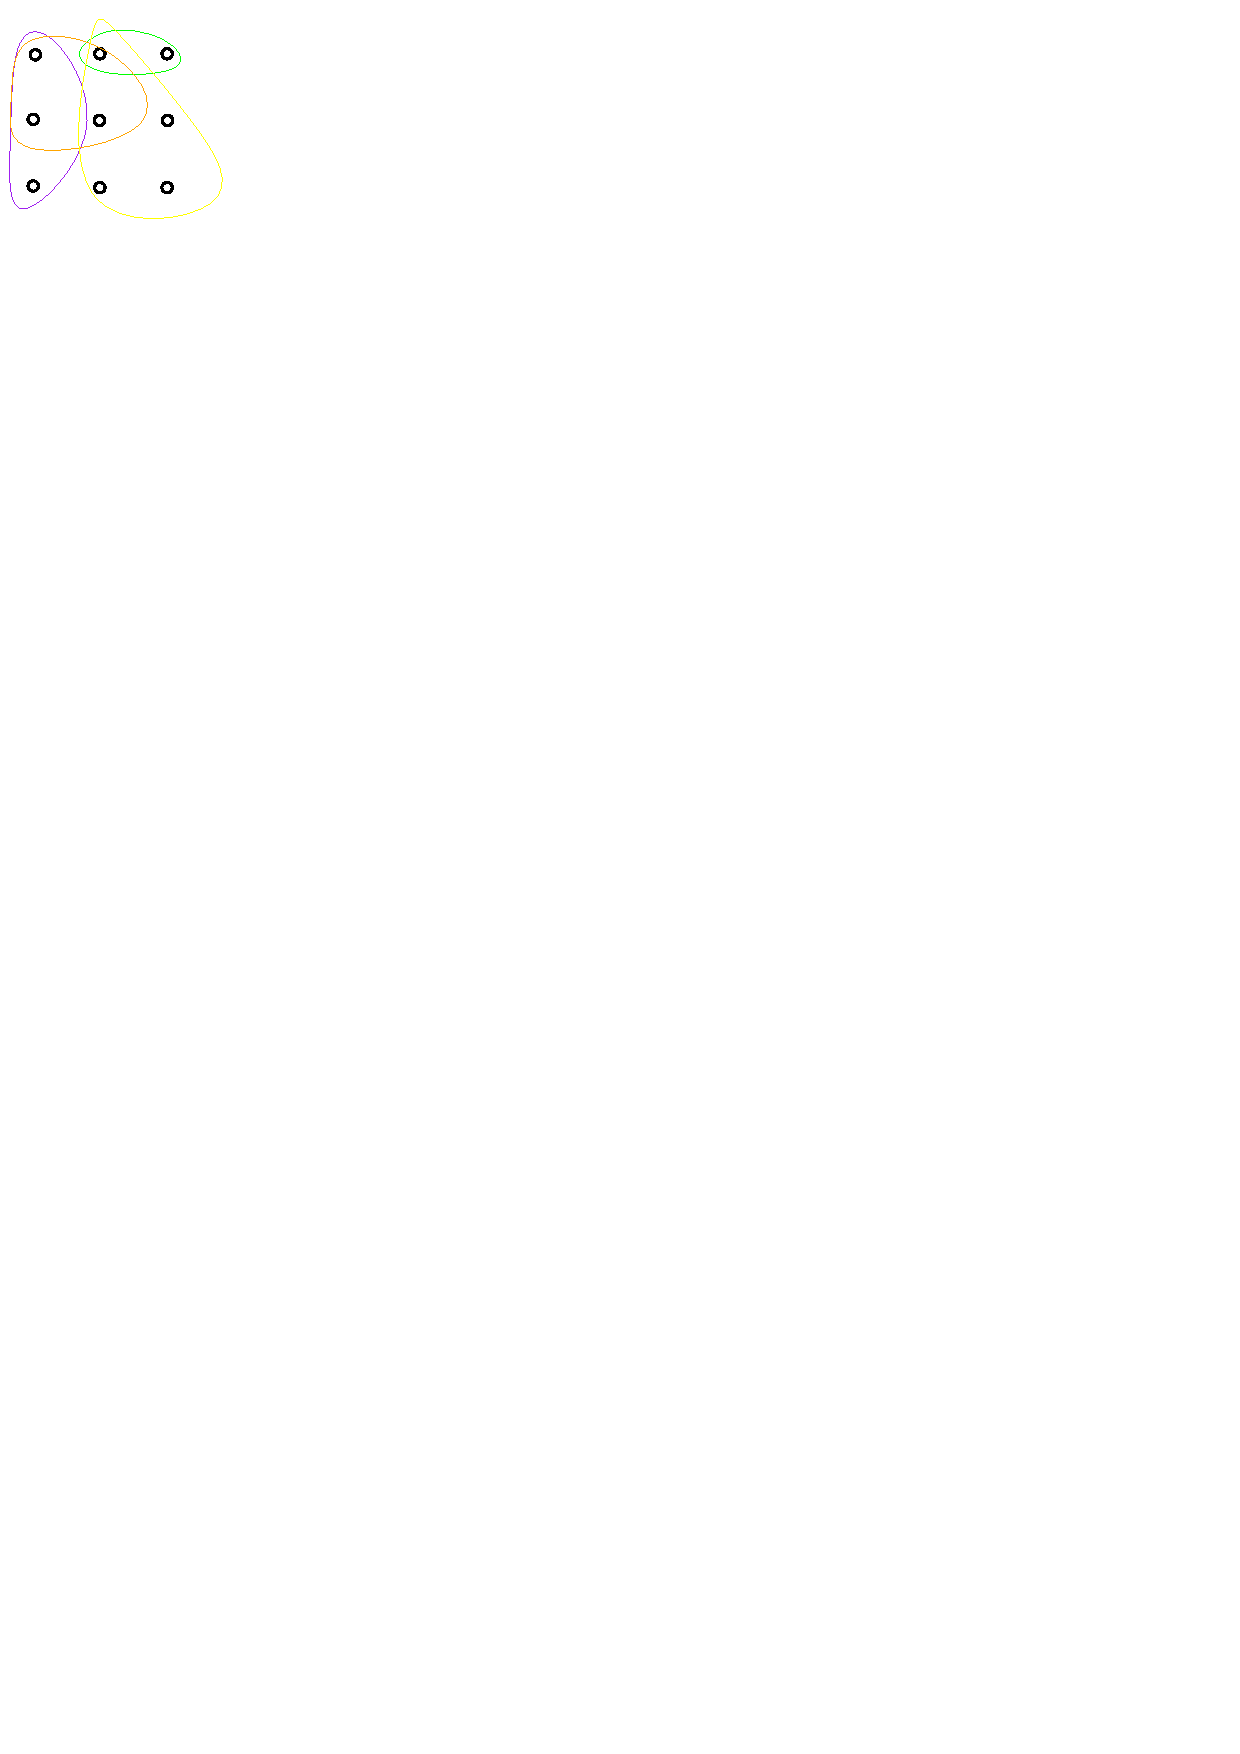
\includegraphics{setsystem}}
    \only<2>{
      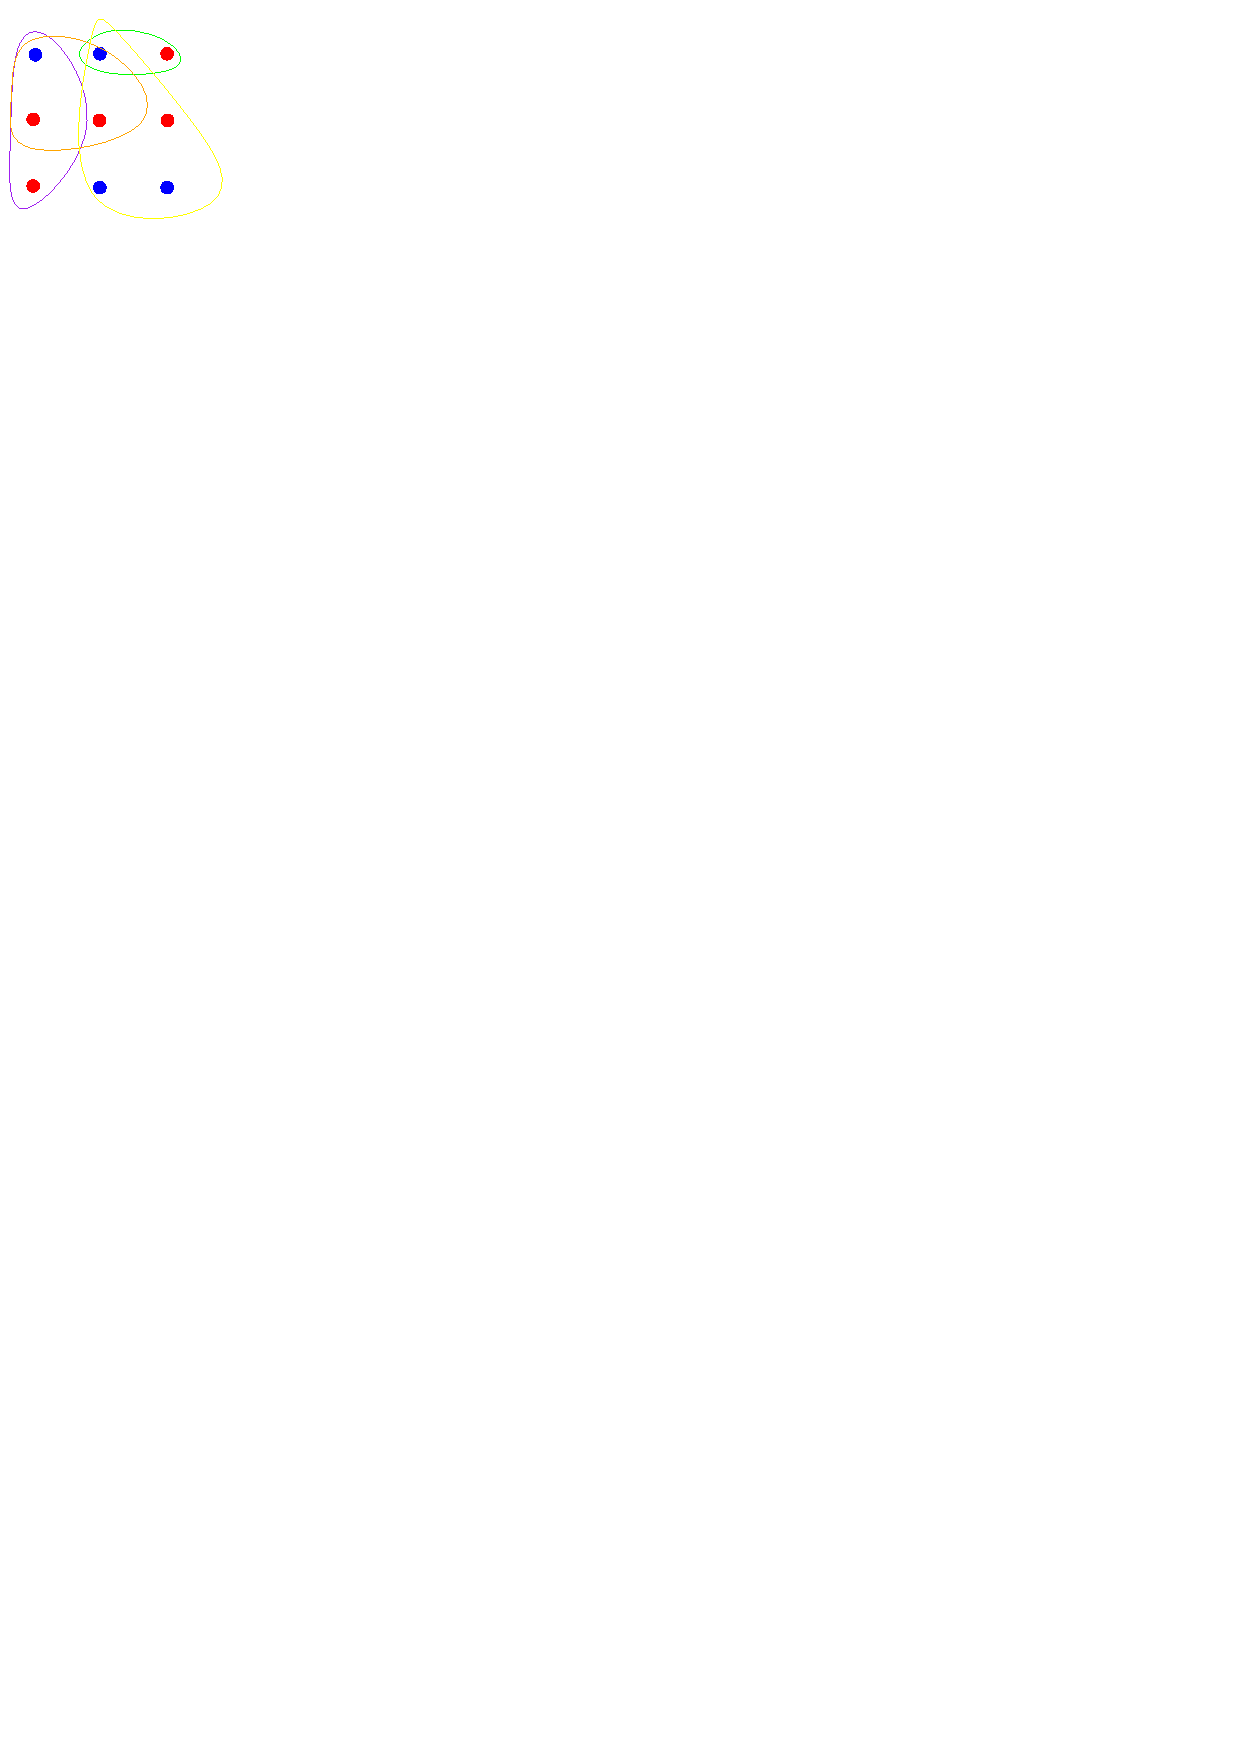
\includegraphics{setsystemcolored}    }
  \end{center}

  Discrepancy of a coloring: maximum imbalance (above: 1). 

  Discrepancy of $\SS$: discrepancy of the best coloring. 



}


\frame{

  \frametitle{Matrix Representation}

  \only<1>{
    \vspace{1.5em}
      \begin{center}
        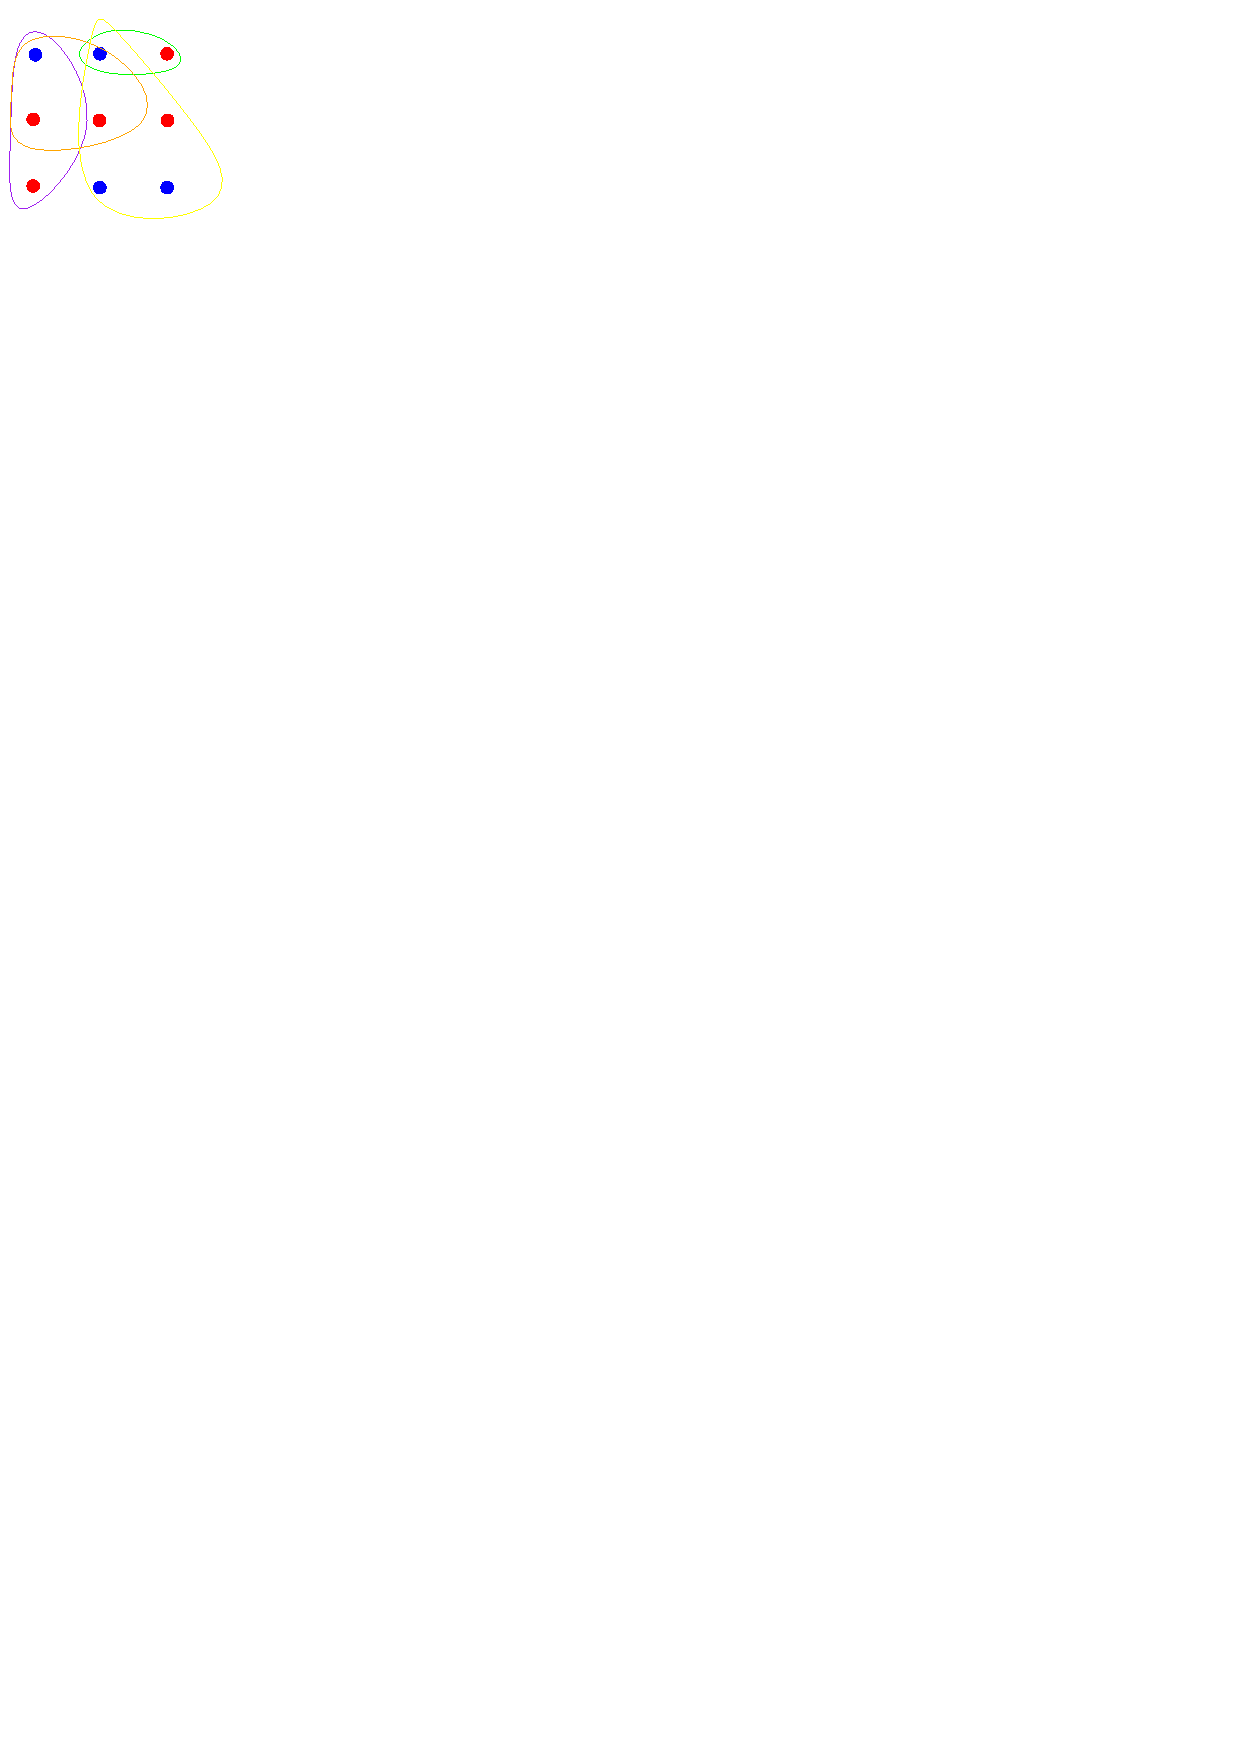
\includegraphics{setsystemcolored}    
      \end{center}
  }
  \only<2>{
    \vspace{1.5em}
      \begin{center}
        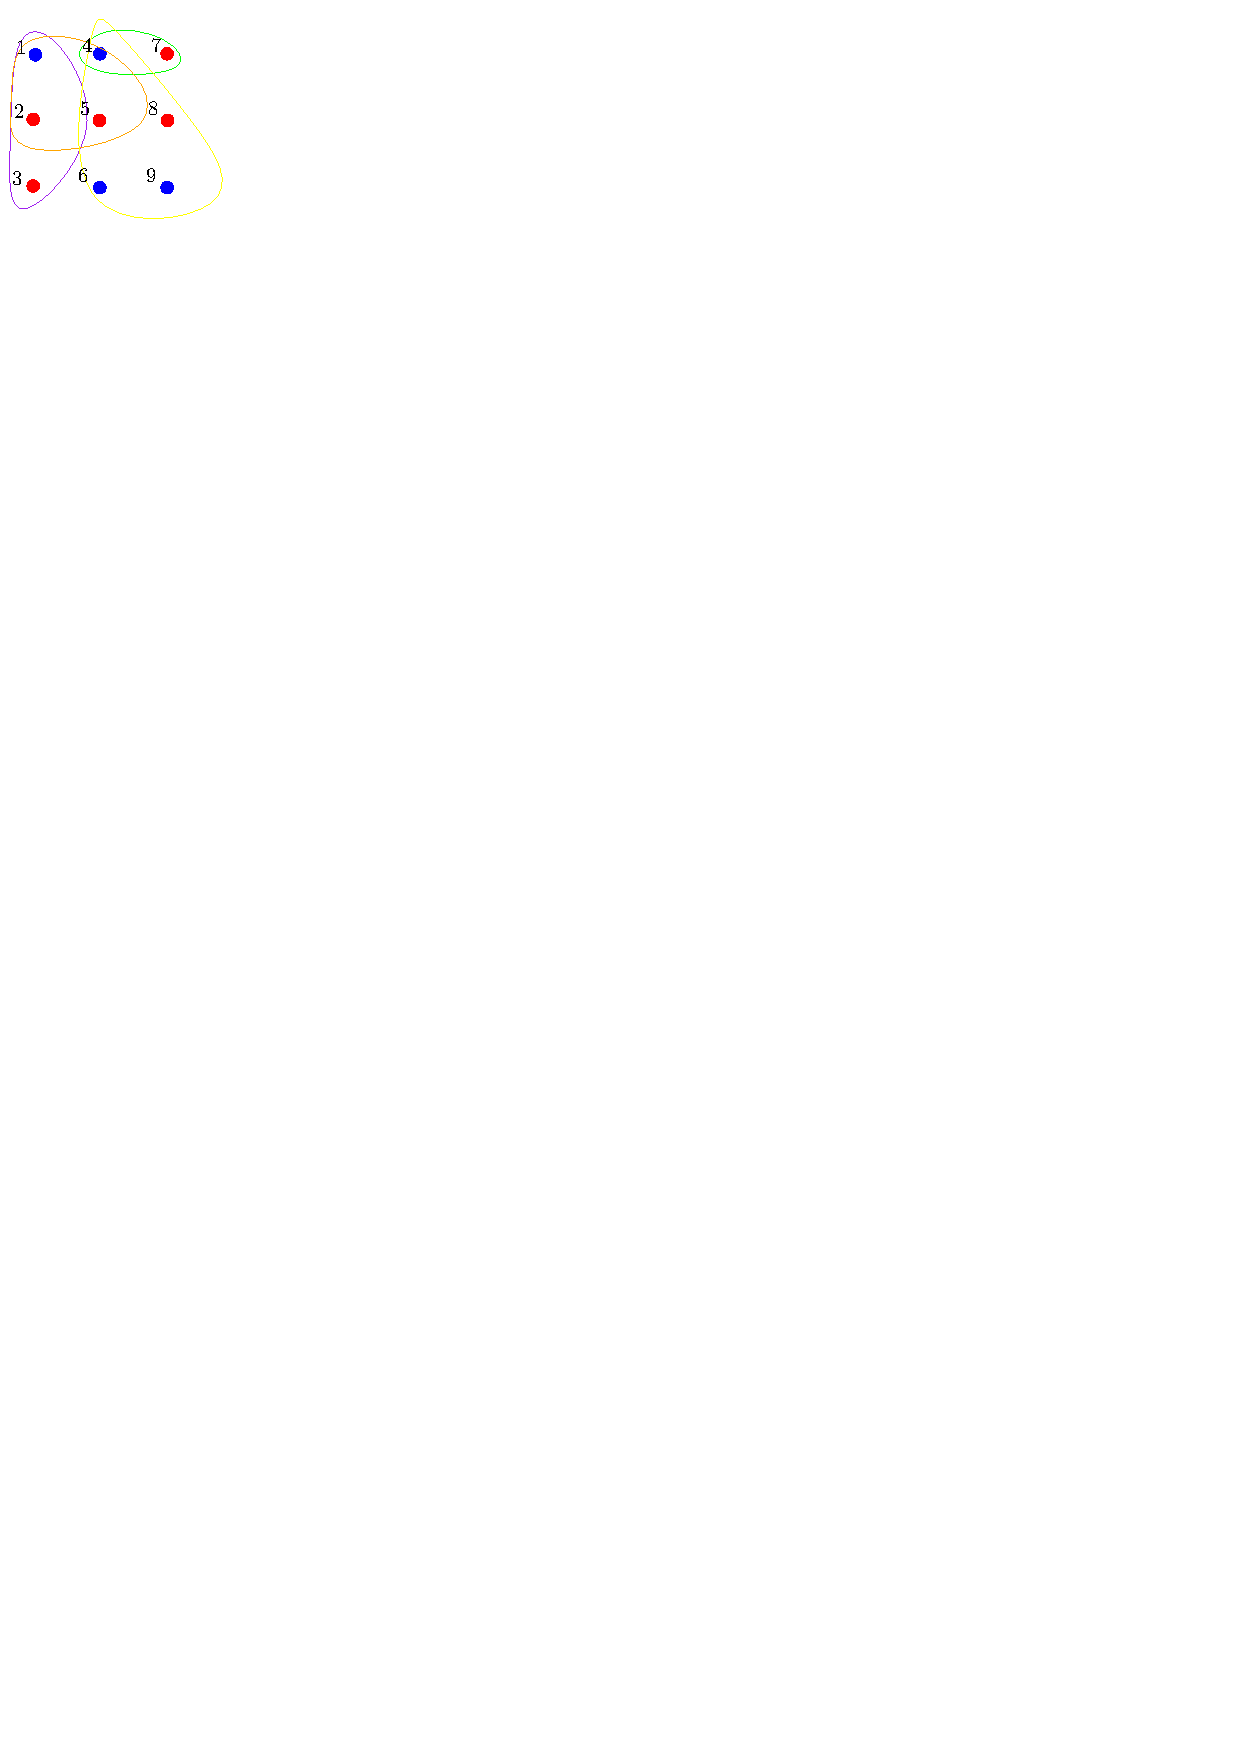
\includegraphics{setsystemnums}    
      \end{center}
  }
  \only<3-4>{
    \begin{align*}
    \left(
      \begin{array}{+c=c=c=c=c=c=c=c=c}
        1 & 2 & 3 & 4 & 5 & 6 & 7 & 8 & 9 \\
        \hline
        \rowstyle{\color{BlueViolet}}
        1 & 1 & 1 & 0 & 0 & 0 & 0 & 0 & 0 \\
        \rowstyle{\color{orange}}
        1 & 1 & 0 & 1 & 1 & 0 & 0 & 0 & 0 \\
        \rowstyle{\color{Lime}}
        0 & 0 & 0 & 1 & 0 & 0 & 1 & 0 & 0 \\
        \rowstyle{\color{yellow}}
        0 & 0 & 0 & 1 & 1 & 1 & 1 & 1 & 1 \\
      \end{array}
    \right) 
    \left(
      \begin{array}{r}
        \color{blue}{-1}\\
        \color{red}{1}\\
        \color{red}{1}\\
        \color{blue}{-1}\\
        \color{red}{1}\\
        \color{blue}{-1}\\
        \color{red}{1}\\
        \color{red}{1}\\
        \color{blue}{-1}\\
      \end{array}
    \right)
    = \left(
      \begin{array}{r}
        \color{red}{1}\\
        0\\
        0\\
        \color{blue}{-1}\\
      \end{array}
    \right)
  \end{align*}
  }
  \only<3>{
    \vspace{4em}
  }
  \only<4>{
    \begin{equation*}
      \disc(\SS) = \disc(U, \|\cdot\|_\infty) = 
      \min_{\eps \in \{\pm 1\}^N}{\|U\eps\|_\infty}
    \end{equation*}
    Natural to consider arbitrary matrices and norms.
  }

}

\junk{\frame{

  \frametitle{Variants}
  
  \textbf{Natural extensions}:
  \begin{itemize}
  \item Discrepancy of an \emph{arbitrary matrix}:\\
    $\disc(U) = \min_{\eps \in \{\pm 1\}^N}{\|U\eps\|_\infty}$. \pause

  \item Discrepancy with respect to an \emph{arbitrary norm} $\|\cdot\|$:
    $\disc(U, \|\cdot\| ) = \min_{\eps \in \{\pm 1\}^N}{\|U\eps\|}$. 
    \begin{itemize}
    \item Studied for $\ell_p$ norms~\mycite{Matousek98-Lp-beckfiala,Larsen17}.
    \end{itemize}\pause
  \end{itemize}
  \medskip

  \textbf{Issues:} Discrepancy is
  \begin{itemize}
  \item not robust to slight changes in the set system
  \item hard to estimate~\mycite{CNN11}
  \end{itemize}\pause
  We need a \emph{robust} version of discrepancy.\pause

  \smallskip
  \textbf{Hereditary Discrepancy} \mycite{LSV}:\\
  $\hd(U, \|\cdot\|) = \max_{S \subseteq [N]} \disc(U_S, \|\cdot\|)$
  \begin{itemize}
  \item $U_S = (u_i)_{i \in S}$.
  \end{itemize}

}}% end junk

\frame{

  \frametitle{Applications}
  
  \begin{itemize}
  \item Constructing uniformly distributed pointsets \mycite{beck-rect}:
    \begin{itemize}
    \item Used in numerical integration (the quasi-Monte Carlo Method);
    \end{itemize}
    \smallskip\pause
    
  \item Constructing {$\epsilon$-nets} \mycite{matousek1995approximations}:
    \begin{itemize}
    \item Used in computational geometry, machine learning;
    \end{itemize}
    \smallskip\pause

  \item Applications in combinatorial optimization: approximation
    algorithms and integrality gaps for
    \begin{itemize}
    \item bin packing~\mycite{HobergRothvoss17,NNN12} and generalizations~\mycite{R12};
    \item {broadcast  scheduling}~\mycite{bcast-scheduling};
    \end{itemize}
    \smallskip\pause
    
  \item Lower bounds for data structures:
    \begin{itemize}
    \item Time to keep dynamic range counts \mycite{disc-larsen};
    \item Space for approximate range counts \mycite{disc-spacelb};
    \end{itemize}
    \smallskip\pause

  \item Algorithms and lower bounds for private data analysis~\mycite{NTZ,smalldb}.
    
  \end{itemize}
}

\frame{

  \frametitle{Basic Bounds}

  \begin{itemize}
  \item \mycite{Spencer, gluskin}: $\disc(\SS) \lesssim  \sqrt{n}$\pause

    \medskip
  \item \emph{Implied by}: For any $u_1, \ldots, u_N \in B_\infty^n = [-1,1]^n$,
    there exist $\eps_1, \ldots, \eps_N \in \{-1, +1\}$ s.t.
    $\|\eps_1 u_1 + \ldots + \eps_N u_N\|_\infty \lesssim
    \sqrt{n}$. \pause

    \bigskip

  \item \mycite{beckfiala}: If every element of $\cal X$ appears in at
    most $t$ sets of $\SS$, then $\disc(\SS) \le 2t - 1$\pause

    \medskip
  \item \emph{Implied by}: For any $u_1, \ldots, u_N \in B_1^n$,
    there exist $\eps_1, \ldots, \eps_N \in \{-1, +1\}$ s.t.
    $\|\eps_1 u_1 + \ldots + \eps_N u_N\|_\infty < 2$. \pause

  \end{itemize}

  \bigskip
  Most combinatorial discrepancy bounds are implied by geometric
  vector balancing arguments. 

}


\frame{

  \frametitle{The Vector Balancing Problem}

  Given $u_1, \ldots, u_N \in \R^n$, and
  symmetric convex body $K\subset \R^n$ ($K = -K$), find the smallest~$t$ such
  that 
  %\vspace{-0.5em}
  \[
  \exists\ \eps_1, \ldots, \eps_N \in \{-1, +1\}: 
  \eps_1 u_1 + \ldots + \eps_N u_N \in tK
  \]

  \begin{center}
    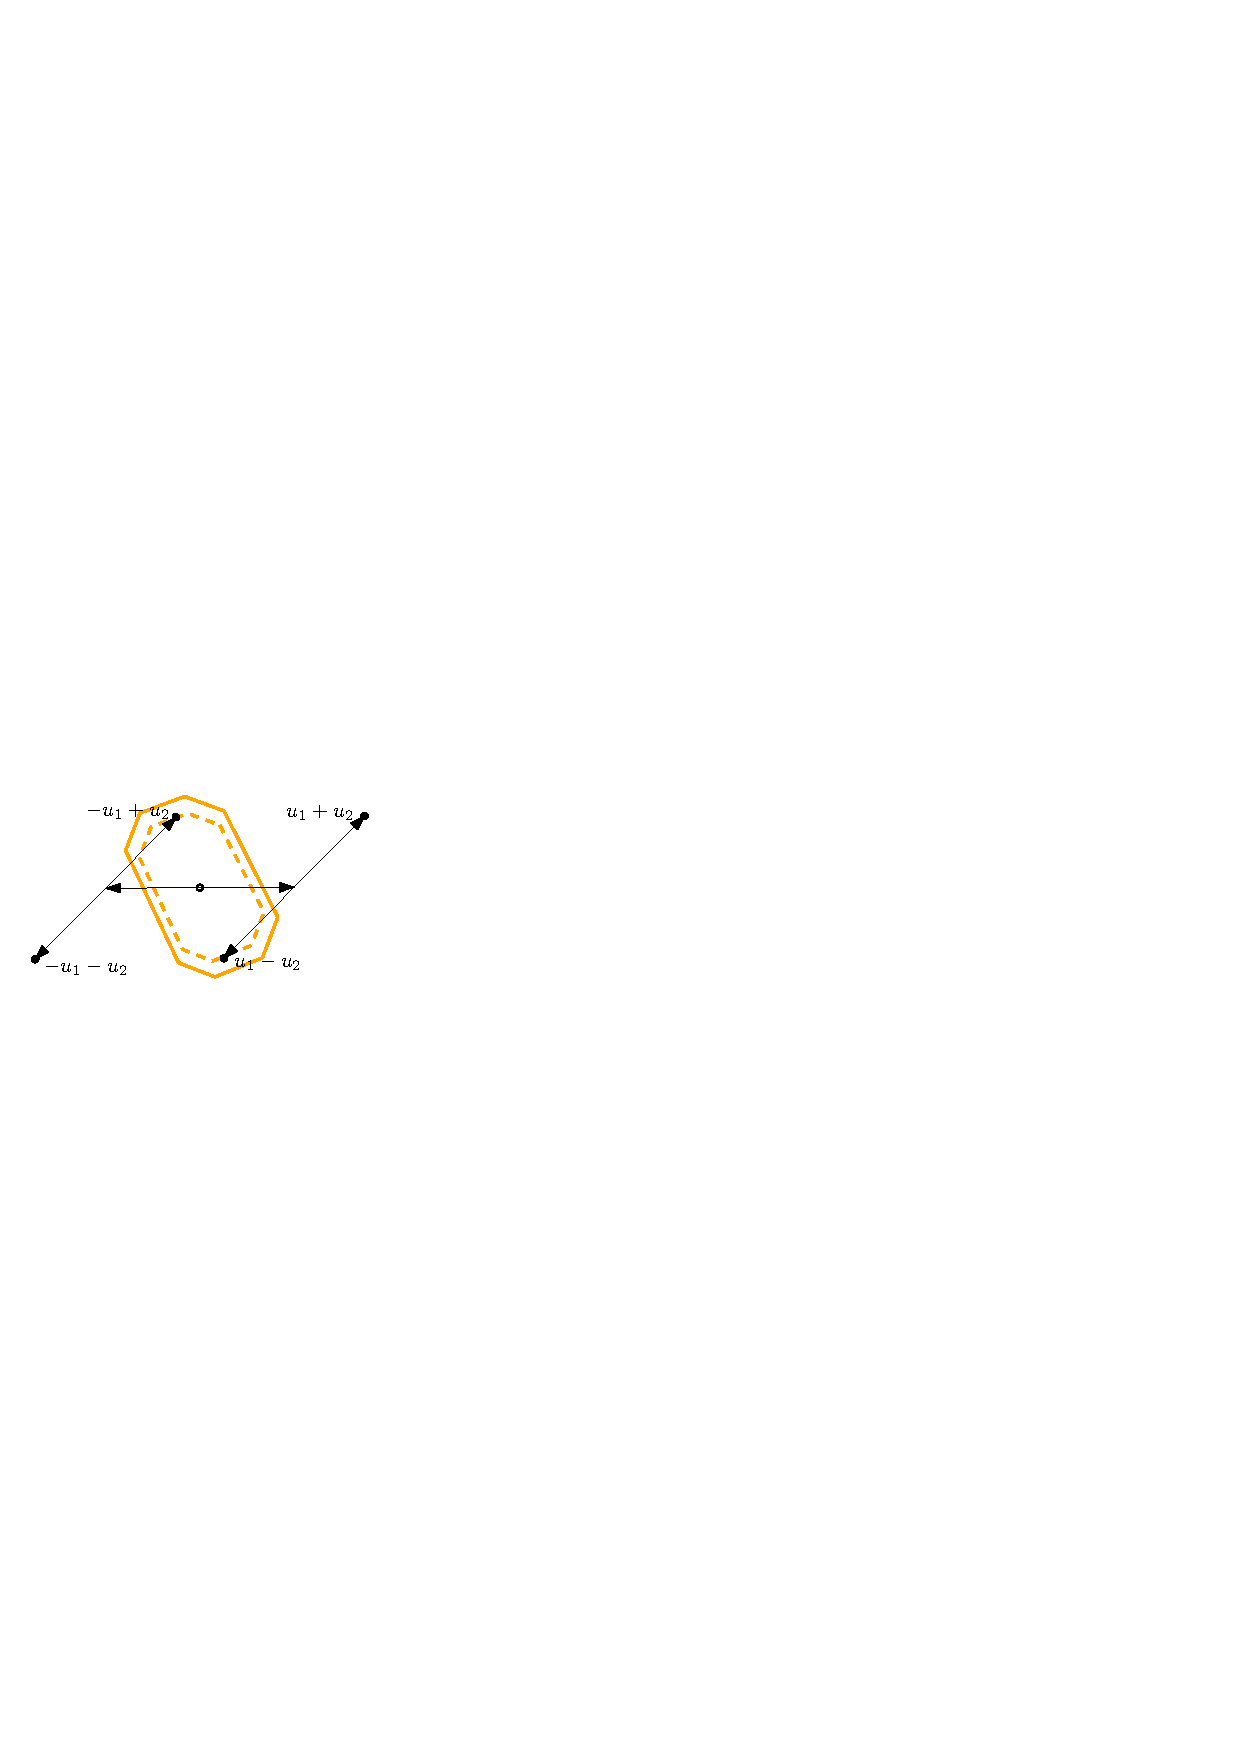
\includegraphics[scale=0.8]{vb}
  \end{center}\pause

  \textbf{Minkowski Norm}: $\|x\|_K = \inf\{t: x \in tK\}$;~$t =
  \disc((u_i)_{i = 1}^N, \|\cdot\|_K)$.\pause

  \smallskip
  \textbf{Vector Balancing Constant}: worst case over
  sequences in $C$
  \begin{align*}
  \vb(C, K) &= 
  %\sup\Bigg\{ 
  %\min_{\eps_1, \ldots, \eps_N \in \{-1,1\}} 
  %\Bigl\|\sum_{i = 1}^N \eps_i u_i \Bigr\|_{K}: 
  %N \in \mathbb{N}, u_1, \ldots, u_N \in C \Bigg\}\\
  %&=
  \sup\Bigg\{ 
  \disc(U, \|\cdot\|_K): 
  N \in \mathbb{N}, u_1, \ldots, u_N \in C, U= (u_i)_{i = 1}^N \Bigg\}
  \end{align*}

}

\frame{

  \frametitle{Questions and Prior Results}

  \begin{itemize}
  \item \mycite{Dvoretzky-problem} ``What can be said'' about
    $\vb(K,K)$?
    
    \smallskip
  \item \mycite{baranygrinberg} $\vb(K, K) \le n$ for all $K$.
    \pause

    \medskip
  \item \mycite{Spencer, gluskin} $\vb(B_\infty^n, B_\infty^n)
    \lesssim \sqrt{n}$\

    \smallskip
  \item \mycite{beckfiala} $\vb(B_1^n, B_\infty^n) < 2$
    \pause

    \medskip
  \item \mycite{bana} $vb(B_2^n, K)\le 5$ if $K$ has Gaussian~measure~$\gamma_n(K) \ge \frac12$

    \smallskip
  \item \emph{Koml\'os Problem}: Prove or disprove $\vb(B_2^n, B_\infty^n) \lesssim 1$.
    \begin{itemize}
    \item Banaszczyk's theorem implies $\vb(B_2^n, B_\infty^n)
      \lesssim \sqrt{\log 2n}$. 
    \end{itemize}
  \end{itemize}

}

\frame{

  \frametitle{Our Results}
  
  We initiate a systematic study of \emph{upper} and \emph{lower
    bounds} on $\vb(C,K)$ and its computational complexity:\pause
  
  \begin{itemize}
  \item A natural volumetric lower bound on $\vb(C,K)$ is
    tight up to a $O(\log n)$ factor.
    \begin{itemize}
    \item The proof implies an efficient algorithm to compute $\eps
      \in \{-1, 1\}^N$ given $u_1, \ldots, u_N \in C$, so that
      $\|\eps_1 u_1 + \ldots + \eps_N u_N\|_K \lesssim (1 + \log n) \vb(C,K)$
    \end{itemize}
\pause

    \medskip
  \item An efficiently computable upper bound on  $\vb(C,K)$ is tight up to
    factors polynomial in $\log n$.
    \begin{itemize}
    \item Based on an optimal application of Banaszczyks' theorem.
    \item Implies an efficient approximation algorithm for $\vb(C,K)$.
    \end{itemize}\pause

    \medskip
  \item The results extend to a robust ``hereditary'' version of
    discrepancy with respect to arbitrary norms.
  \end{itemize}\pause

  Prior work~\mycite{Bansal10,NT15} implies bounds which deteriorate
  with the number of facets of $K$.
}

\section{Volume Lower Bound}

\frame{

  \frametitle{Hereditary Discrepancy}

  \textbf{Issue}: $\disc(U, K) = \disc(U,\|\cdot\|_K)$ is
  \begin{itemize}
  \item not robust to slight changes in $U$ (e.g.~repeat each column)
  \item hard to approximate~\mycite{CNN11}
  \end{itemize}\pause

  \medskip
  $\vb(C,K)$ is more robust, but not about a
  specific matrix $U$.\pause

  \medskip
  \textbf{Hereditary discrepancy} is a robust analog of discrepancy:
  \[
  \hd(U, K)  = \max_{S \subseteq [N]} \disc(U_S, K),
  \]
  where $U_S = (u_i)_{i \in S}$ is the submatrix of $U$ indexed by
  $S$. \pause

  \smallskip
  \textbf{Observation}: 
  \[
  \vb(C, K) = \sup\Bigg\{ 
  \hd(U, K): 
  N \in \mathbb{N}, u_1, \ldots, u_N \in C, U = (u_i)_{i = 1}^N \Bigg\}.
  \]

}

\frame{

  \frametitle{The Volume Lower Bound}

  \only<1>{\vspace{-6em}}
  Define $L = \{x \in \R^N: Ux \in K\}$: the set of ``good $x$''.
  \begin{itemize}
  \item $\disc(U, K) = \min\{t: tL \cap \{-1,1\}^N \neq \emptyset\}$.
  \end{itemize}\pause
  
  \mycite{LSV}: \\
  If $t = \hd(U, K)$, 
  then $[0,1]^N \subseteq \bigcup_{x \in \{0,1\}^N}\left(x +  t L\right)$.
  \only<2>{
    \begin{center}
      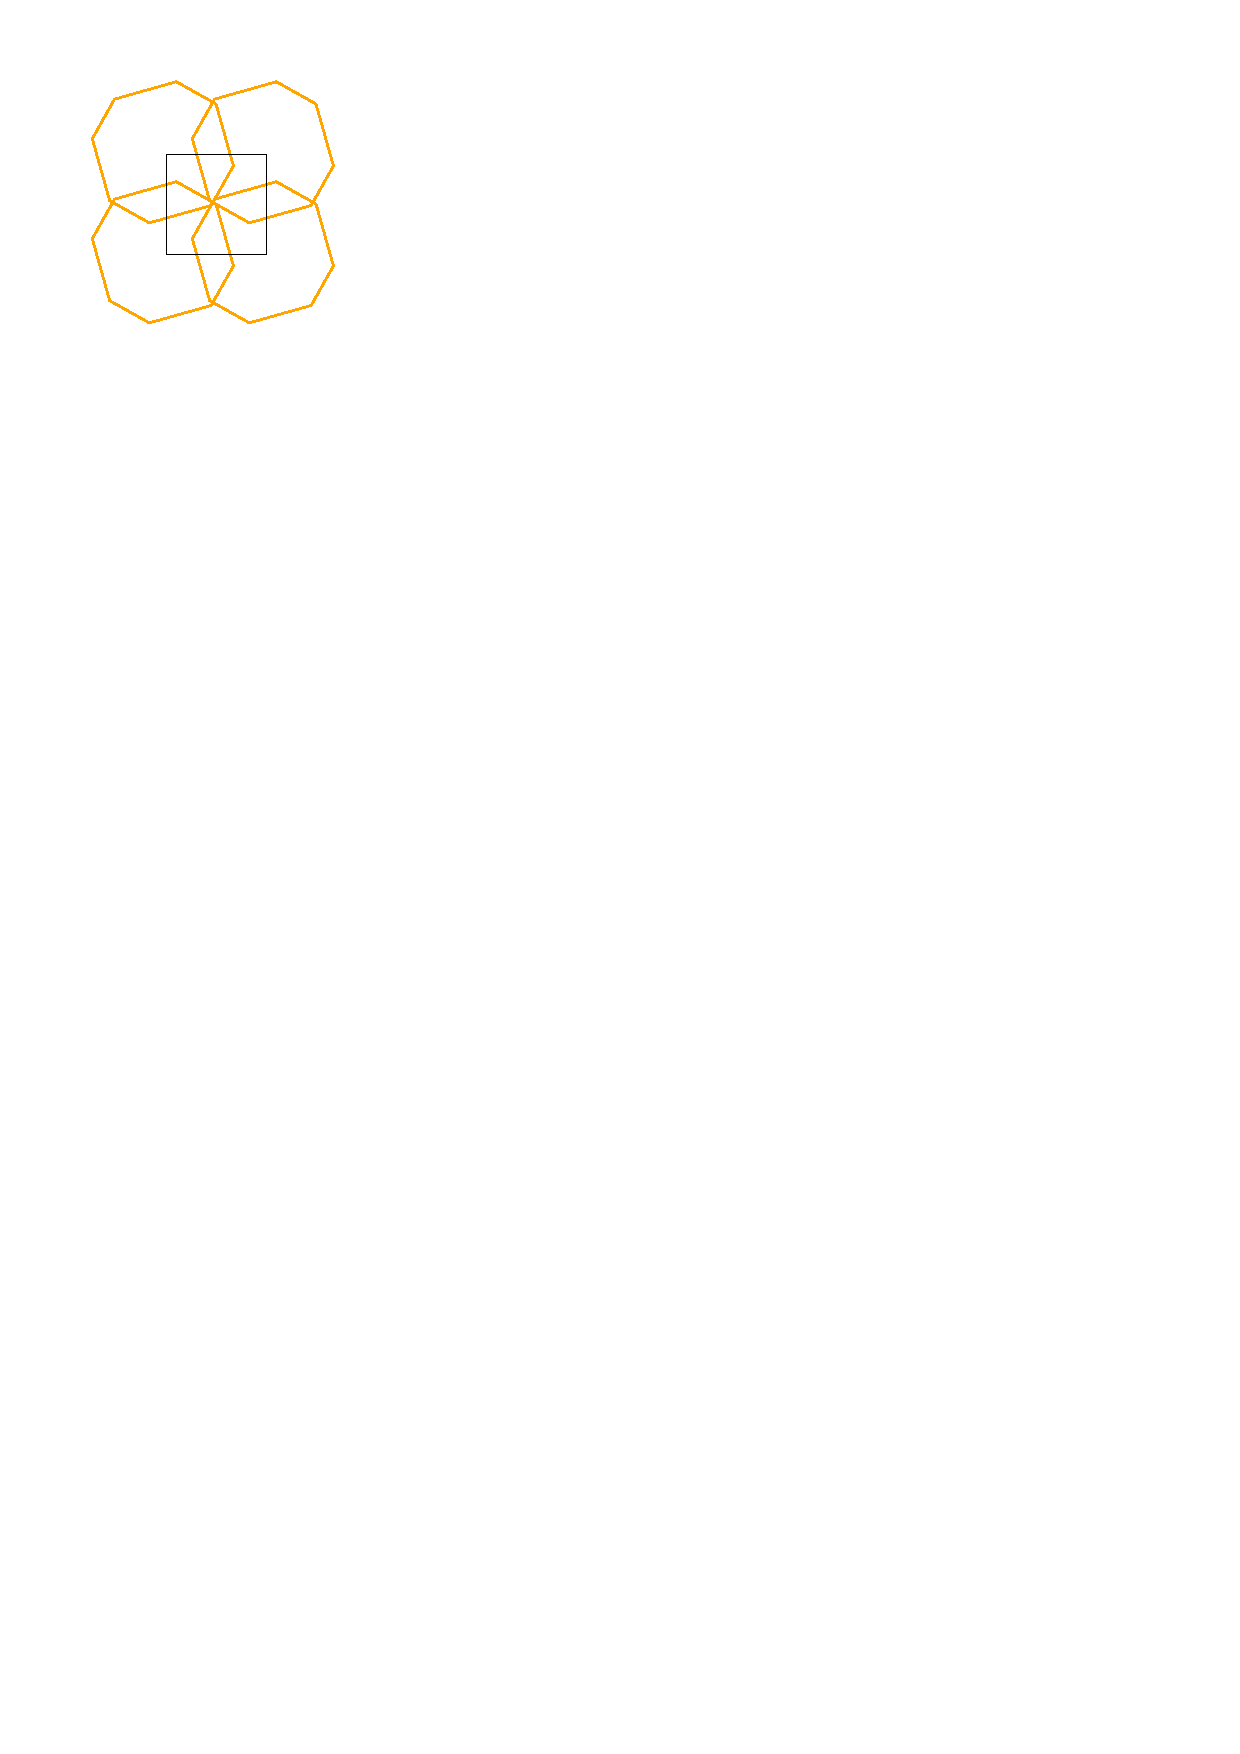
\includegraphics[scale=0.7]{volLB}
    \end{center}
  }\pause
  \only<3->{
    \begin{center}
      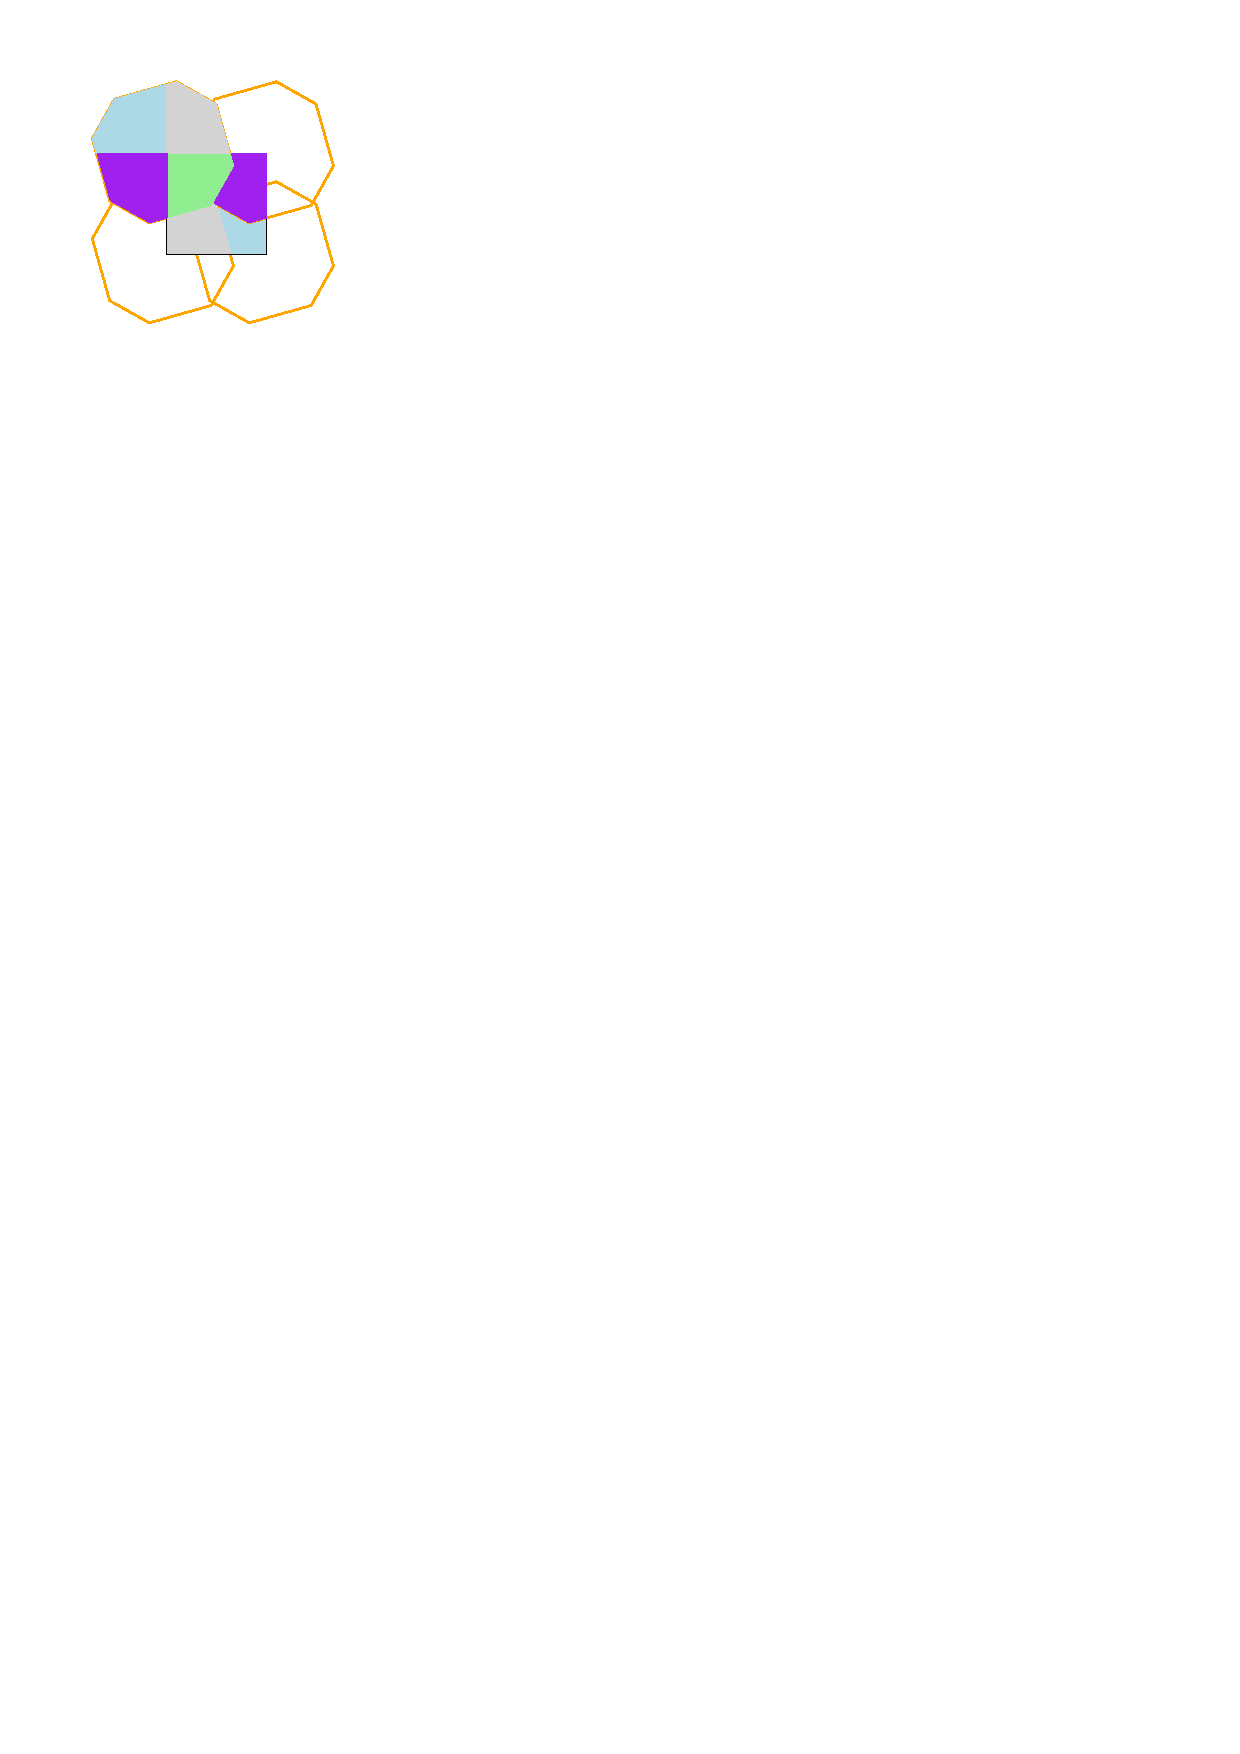
\includegraphics[scale=0.7]{volLB-colors}
    \end{center}
  }
  
  \mycite{Bana93}:
  \[
  1 = \vol([0,1]^N) \ge \vol(t L) = t^N \vol(L)
  \only<3>{\hspace{13em}}
  \only<4>{\iff
  \hd(U,K) \ge {\vol(L)^{-1/N}}.}
  \]
}

\frame{

  \frametitle{A Hereditary Volume Lower Bound}
  
  A simple strengthening:
  \[
  \hd(U, K) \ge \vollb(U, K) 
  = \max_{S \subseteq [N]} \vol(\{x \in \R^S: U_Sx \in K\})^{-1/|S|}.
  \]\pause

  \medskip
  Lower Bound on $\vb(C,K)$:
  \begin{align*}
  \vb(C,K) &\ge \vollb(C,K) 
  = \sup\Bigl\{\vollb((u_i)_{i=1}^N,K): u_1, \ldots, u_N \in C\Bigr\}.
  \end{align*}\pause

  \begin{theorem}
    For any $n \times N$ matrix $U$, and any symmetric convex $C, K
    \subset \R^n$,
    \vspace{-1em}
    \begin{align*}
    \vollb(U,K) &\le \hd(U, K) \lesssim (1+\log n)\cdot \vollb(U,K)\\
    \vspace{0.5em}
    \vollb(C,K) &\le \vb(C, K) \lesssim (1+\log n)\cdot \vollb(C,K)
    \end{align*}
  \end{theorem}

}

\frame{
  
  \frametitle{Rothvo\ss's Algorithm}
  
  \begin{columns}
    \column{0.7\linewidth}
    Algorithm~\mycite{rothvoss-giann}: given $K \subset \R^n$,
    \begin{enumerate}
    \item Sample a standard Gaussian $G \sim N(0,I_n)$;
    \item Output \\$X = \arg \min\{\|x - G\|_2^2: x \in K \cap [-1,1]^n\}$.
    \end{enumerate}
  
    \column{0.3\linewidth}
    \begin{center}
      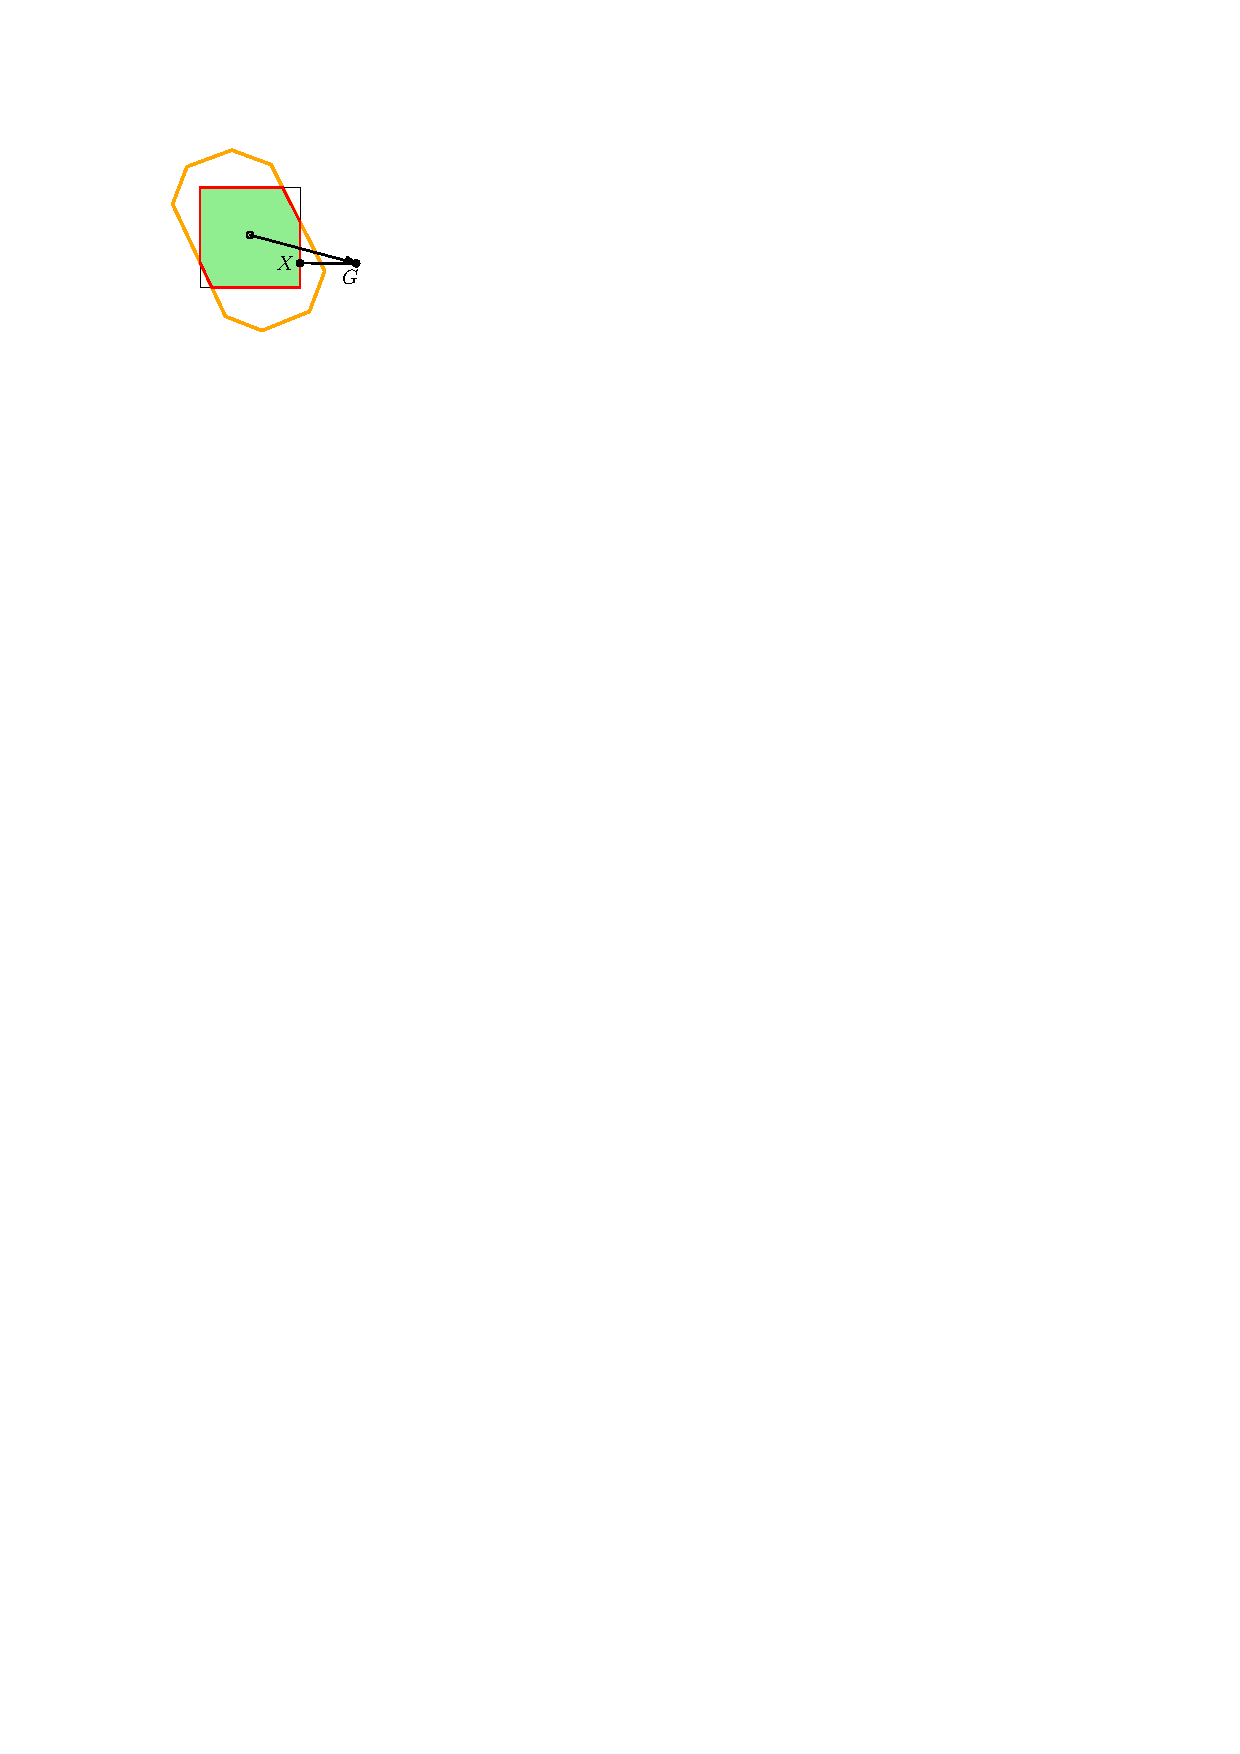
\includegraphics[scale=0.8]{R-alg}
    \end{center}
  \end{columns}

  \textbf{Goal}: $|\{i: X_i \in \{-1, +1\}\}| \ge \alpha n$ for a constant $\alpha$.\\
  ($X$ is a \emph{partial coloring}.)

  \smallskip
  \textbf{Intuition}: If $K$ is ``big enough,'' then in an average direction
  $\partial [-1,1]^n$ is closer to the origin than $\partial K$ and is
  more likely to be hit by $X$.\pause
  \only<1>{\vspace{4.8em}}
  
  \smallskip 
  \only<2>{
    \mycite{rothvoss-giann} For any small enough $\alpha$
    there is a $\delta$ so that \\
    if $K$ has Gaussian measure $\gamma_n(K) \ge e^{-\delta n}$, then\\
    with high probability $|\{i: X_i \in \{-1, +1\}| \ge \alpha n$. 
    \vspace{1.2em}
  }
  \only<3>{
    \mycite{rothvoss-giann} For any small enough $\alpha$
    there is a $\delta$ so that \\
    \emph{if there exists a dimension $(1-\delta)n$
      subspace $W$ for which} \\
    $K \cap W$ has Gaussian measure  $\gamma_W(K \cap W)    \ge e^{-\delta n}$, then\\ 
    with high probability $|\{i: X_i \in \{-1,    +1\}\}| \ge \alpha n$.  
  }

}

\frame{

  \frametitle{Tightness of the Volume Lower Bound}

  Need to show: for any $U \in \R^{n \times N}$ and symmetric convex
  $K \subset \R^n$
  \vspace{-0.5em}
  \[
  \hd(U, K) \lesssim (1+\log n)\cdot \vollb(U,K).
  \vspace{-0.5em}
  \]\pause
  Proof by an algorithm: \\
  Find a partial coloring with discrepancy $\lesssim \vollb(U,K)$ and recurse.\pause
  \begin{enumerate}
  \item Preprocess so that $N = n$, $U = I_n$;
  \item Apply Rothvo\ss's algorithm to $t K$, 
    $t \asymp  \vollb(I_n,K)$; 
    \begin{itemize}
    \item \emph{If conditions hold}, gives a partial coloring $X \in
      t K$;
    \end{itemize}
    
  \item $S = \{i: -1 < X_i < 1\}$; Project $K$ on $\R^S$ and recurse.
    \begin{itemize}
    \item Need a ``recentered'' variant of Rothvo\ss's algorithm.
    \end{itemize}
  \end{enumerate}\pause

  \smallskip
  After $k \lesssim 1+\log n$ iterations, we have $X^1, \ldots X^k$ so
  that 
  \vspace{-0.5em}
  \begin{align*}
    X^1 + \ldots + X^k &\in \{-1,1\}^n;\\
    \|X^1 + \ldots + X^k\|_K &\le kt \lesssim (1+\log n)\vollb(I_n,K).
  \end{align*}\pause

  \vspace{-2em}
  \textbf{Main Challenge}: Show that the conditions of Rothvo\ss's
  algorithm are satisfied.
}

\frame{

  \frametitle{From Volume To Gaussian Measure}

  For Rothvo\ss's algorithm, we need that on some subspace of large
  dimension, the body $tK$, $t\asymp \vollb(I_n,K)$, has large Gaussian measure.\pause

  \smallskip
  From the definition of $\vollb(I_n, K)$:
  \vspace{-0.5em}
  \begin{equation*}%\label{eq:vol-sect}
  \forall S \subseteq [n]: 
  \vol((\vollb(I_n,K)\cdot K) \cap \R^S) \ge 1.
  \end{equation*}\pause

  
  \begin{theorem}[Structural result]
    For any $\delta$ there exists a $m = m(\delta)$ so that the
    following holds.\\
    Let $L$ be a symmetric convex body s.t.~$\vol(L \cap \R^S) \ge 1$
    for all $S \subseteq [n]$. \\
    There exists a subspace $W$ of dimension $(1-\delta) n$ for which
    \vspace{-0.5em}
    \[\gamma_W((m L) \cap W) \ge e^{-\delta n}.\]
  \end{theorem}
  Apply to $L = \vollb(I_n,K)\cdot K$ to get that the conditions of
  Rothvo\ss's algorithm are satisfied. 

}

\frame{

  \frametitle{Proof Ideas}

  Generally applicable strategy:
  \begin{enumerate}
  \item Prove the theorem for an ellipsoid $E = T(B_2^n)$.
    \begin{itemize}
    \item Reduces to linear algebra!
    \end{itemize}\pause

  \item Approximate a general convex body $L$ by an appropriate
    ellipsoid. 

    \begin{theorem}[Regular $M$-ellipsoid, \mycite{Milman86-reverseBM,Pisier89}]
      For any symmetric convex $L \subseteq \R^n$ there exists an
      ellipsoid $E$ such that 
      \vspace{-0.7em}
      \[
      \max\{N(L, tE), N(E, tL)\} \le e^{cn/t},
      \vspace{-0.7em}
      \]
      where $c$ is a constant.
    \end{theorem}
    \noindent
     $N(K,L)=$  number of  translates of $L$ needed to cover $K$.\\
     $E$ preserves ``large scale'' information about $L$.
  \end{enumerate}\pause

  \begin{itemize}
  \item $L\cap \R^S$ has large volume $\implies$
    $E \cap \R^S$ has large volume.
  \item $E \cap W$ has large Gaussian measure $\implies$
    $L \cap W$ has large Gaussian measure.
  \end{itemize}
}

\frame{

  \frametitle{Partial Colorings}

  The bound $\hd(U,K) \lesssim (1+\log n) \vollb(U,K)$ is in
  general tight.\pause

  \smallskip
  Is the hereditary discrepancy of partial
  colorings $\asymp \vollb(U,K)$?\pause
  \begin{itemize}
  \item The hereditary discrepancy of partial colorings is
    $\lesssim \vollb(U,K)$.\pause
  \item A lower bound would follow from
    \begin{conjecture}
      Suppose $K \subset \R^n$ is a symmetric convex body of volume
      $\le 1$. Then there
      exists a $S \subseteq [n]$ s.t.~$\mathrm{diam}_{\ell_2}(K \cap \R^S)
      \lesssim \sqrt{|S|}$. 
    \end{conjecture}\pause
    \item True for ellipsoids and reduces to the Restricted
      Invertibility Principle.
    \item True for general bodies $K$ if we replace $\R^S$ with an
      arbitrary subspace $W$ and $|S|$ with $\mathrm{dim}\ W$.
  \end{itemize}

}

\section{Factorization Upper Bounds}

\frame{
  
  \frametitle{Upper Bounds from Banaszczyk's Theorem}

  We showed how to efficiently compute near optimal signs $\eps_1,
  \ldots, \eps_N \in \{-1,1\}$ for any $u_1, \ldots, u_N$.

  \smallskip
  But what if we want to compute $\vb(C,K)$ or $\hd(U,K)$?\pause
  \begin{itemize}
  \item We do not know how to efficiently compute $\vollb(C,K)$.
  \item We need a natural \emph{upper bound} on $\vb(C,K)$.
  \end{itemize}\pause

  %\smallskip
  Recall \mycite{bana}:\\ For any convex $K \subset \R^n$ such that
  $\gamma_n(K) \ge \frac12$, $\vb(B_2^n, K) \le 5$.\pause

  \smallskip
  \textbf{Observations}:
  \begin{itemize}
  \item If $\E \|G\|_K\le 1$ for $G \sim N(0,I_n)$, then
    $\gamma_n(2K) \ge \frac12$. 
  \item $\vb(B_2^n, K) \lesssim \E \|G\|_K$. \pause
    \smallskip
    
  \item $\vb(C, K) \lesssim (\E \|G\|_K) \cdot
    \mathrm{diam}_{\ell_2}(C)$.
  \end{itemize}
  Last bound can be very loose! Can we do better?

}

\frame{
  
  \frametitle{A Better Upper Bound}

  \textbf{Idea}: Map $C$ into $B_2^n$ using a linear map.
  \[
  \lambda(C,K) = 
  \inf\{ (\E \|G\|_{T(K)})\cdot \mathrm{diam}_{\ell_2}(T(C)):
  T \text{ a linear map}\}.
  \]
  \textbf{Claim}: $\vb(C,K) \lesssim \lambda(C,K)$.\pause

  \smallskip
  \begin{itemize}
  \item Take a linear map $T$ achieving $\lambda(C, K)$;
    \begin{itemize}
    \item Can assume $\mathrm{diam}_{\ell_2}(T(C)) = 1$, 
      so $\E \|G\|_{T(K)} = \lambda(C,K)$;
    \end{itemize}\pause
  \item $\vb(C,K) = \vb(T(C), T(K))$ and apply Banaszczyk's theorem.
  \end{itemize}
  
}

\frame{
  \frametitle{Tightness of the Upper Bound}

  \begin{theorem}
    For any symmetric convex $C, K \subset \R^n$,
    \vspace{-1em}
    \begin{align*}
      \frac{\lambda(C,K) }{(1+\log n)^{5/2}} 
      \lesssim \vb(C, K) 
      \lesssim \lambda(C,K).
    \end{align*}
    Moreover, given membership oracle access to $K$ and a vertex
    representation of $C$, we can efficiently compute $\lambda(C,K)$. 
  \end{theorem}
  
  For a matrix $U \in \R^{n \times N}$, we can take $C = \conv\{\pm
  u_1, \ldots, \pm u_N\}$, and then $\lambda(C,K)$ approximates
  $\hd(U,K)$. \pause

  \smallskip
  \textbf{Proof outline}:
  \begin{enumerate}
  \item Formulate $\lambda(C,K)$ as a convex minimization problem;
  \item Derive the Lagrange dual: an equivalent maximization problem;
    %\begin{itemize}
    %\item Dual solutions give lower bounds on $\lambda(C,K)$;
    %\end{itemize}
  \item Relate dual solutions to the volume lower bound. 
  \end{enumerate}
}

\frame{
  \frametitle{Convex Formulation}

  $\|x\|_{T(K)} = \|T^{-1}x\|_K$

  \smallskip
  \textbf{First attempt}: $\inf\{\E \|T^{-1}G\|_K:
  \mathrm{diam}_{\ell_2}(T(C)) \le 1\}$
  \begin{itemize}
  \item \emph{Not convex}: the objective is $\infty$ for $T = 0$ and
    finite for any invertible $T$, but $0 = \frac12(T + (-T))$. 
  \end{itemize}\pause

  \smallskip
  \textbf{Observation}: $\E \|T^{-1}G\|_K$ is defined
  entirely by $A = T^*T$, because the covariance of
  $T^{-1}G$ is given by $A^{-1}$. \pause

  \smallskip
  \textbf{Formulation}:
  \vspace{-2em}
  \begin{align*}
    \lambda(C,K) = &\inf  f(A) \\
    \text{s.t.\ \ }
    &\langle x, Ax\rangle \le 1 \ \ \ \forall x \in C\\
    &A \succ 0.
  \end{align*}
  
  \vspace{-1em}
  \begin{itemize}
  \item $f(A) = \E \|T^{-1}G\|_K$ for any $T$ such that
    $T^*T = A$;
    \begin{itemize}
    \item $f$ is well defined over positive definite $A$;
    \end{itemize}\pause

  \item The first constraint encodes $\mathrm{diam}_{\ell_2}(T(C)) \le
    1$: 
    $\langle x, Ax\rangle = \langle x, T^* T x\rangle 
    = \langle Tx, Tx\rangle = \|Tx\|_2^2$.
  \end{itemize}

}

\frame{
  
  \frametitle{Properties of the Formulation}
  
  \begin{itemize}
  \item The function $f(A)$ is convex in $A$, and the constraints are
    also convex;

  \item \textbf{Lagrange Duality}: there exists an
    \emph{equivalent} dual maximization problem, whose value also equals
    $\lambda(U,C)$;\pause

  \item Each dual solution gives a lower bound on $\vollb(C,K)$, and,
    therefore, on $\vb(C,K)$;
    \begin{itemize}
    \item Tools: $K$-convexity, and Sudakov minoration;
    \end{itemize}

  \item $\implies$ $\lambda(C,K)$ gives a lower bound on $\vb(C,K)$.
  \end{itemize}\pause

  \textbf{Computation}: The convex optimization problem can be solved
  using the ellipsoid method, given a membership oracle for $K$ and a
  vertex representation of $C$.
  
}

\section{Conclusion}

\frame{

  \frametitle{Conclusion}

  \textbf{In this work}:
  \begin{itemize}
  \item Tightness of natural upper and lower bounds for vector
    balancing.

  \item Efficient algorithms to find nearly optimal vector balancing
    signs, and to compute $\vb(C,K)$, and hereditary discrepancy with
    respect to any norm. 

  \item Our results strongly use the geometry of the underlying
    discrepancy problem. 
  \end{itemize}\pause

  \textbf{Open questions}:
  \begin{itemize}
  \item Does $\vollb(C,K)$ give lower bounds on partial colorings?
  \item $\vb(K,K) \asymp \vollb(K,K)$? (True for $\ell_p$.)
  \item Can the bounds for $\lambda(C,K)$ be improved?
  \end{itemize}
}

\bibliographystyle{plainnat}
\bibliography{../Discrepancy}

\end{document}


